%
% simplex.tex -- simplizes und Polyeder
%
% (c) 2021 Prof Dr Andreas Müller, OST Ostschweizer Fachhochschule
%
\section{Simplizes
\label{buch:section:simplexe}}
\rhead{Simplizes}
Die Idee, das Dreieck und seinen Rand zu unterscheiden verlangt,
dass wir zunächst Dreiecke und deren höherdimensionale Verallgemeinerungen,
die sogenannten Simplizes entwickeln müssen.

\subsection{Simplizes und Rand
\label{buch:subsection:simplices}}

\subsubsection{Rand eines Dreiecks}
Die Inzidenz-Matrix eines Graphen hat einer Kante die beiden Endpunkte
mit verschiedenen Vorzeichen zugeordnet.
Dieses Idee soll jetzt verallgemeinert werden.
Der Rand des Dreiecks $\triangle$ in
Abbildung~\ref{buch:homologie:figure:zusammenziehbar}
besteht aus den Kanten $P_0P_1$, $P_1P_2$ und $P_0P_2$.
Für eine algebraische Definition müssen die Kanten offenbar eine
Orientierung haben, die ist aber garantiert, da wir den Anfangs-
und Endpunkten einer Kante verschiedene Vorzeichen gegeben haben.
Dem Dreieck $\triangle$ werden dann die drei Kanten $k_{01}$, $k_{02}$
und $k_{12}$ zuogeordnet, aber mit zusätzlichen Vorzeichen, die
die Orientierung festhalten.
Durchläuft man den Rand von $\triangle$ in der Reihenfolge $P_0P_1P_2$,
dann müssen die Kanten $k_{12}$ und $k_{02}$ ein negatives Vorzeichen
erhalten.

Wir können diese Zuordnung wieder mit einer Matrix ausdrücken.
\[
\begin{matrix}
\text{$k_{01}$:}\mathstrut\\
\text{$k_{02}$:}\mathstrut\\
\text{$k_{12}$:}\mathstrut
\end{matrix}
\qquad
\partial
=
\begin{pmatrix*}[r]
1\mathstrut\\
-1\mathstrut\\
1\mathstrut
\end{pmatrix*}
\]

\subsubsection{Simplizes}
Punkte, Kanten und Dreiecke sind die einfachsten Fälle sogenannter
Simplizes.
Wir formulieren die Definition dieser Objekte auf eine Weise,
die uns ermöglichen soll, sie auf beliebige Dimension zu verallgemeinern.

Die Strecke, die die Punkte $P$ und $Q$ miteinander verbindet,
kann beschrieben werden durch eine Parametrisierung
der Form
\begin{equation}
s_1
\colon
t
\mapsto
t\vec{p} + (1-t) \vec{q}
=
t_0 \vec{p} + t_1\vec{q},
\end{equation}
wobei die beiden positiven reellen Zahlen $t_0,t_1\in\mathbb{R}$ die
Bedingung $t_0 + t_1 = 1$ erfüllen.
Für ein eindimensionales Objekt brauchen wir also zwei Punkte und zwei
positive Parameter, die sich zu $1$ summieren.
Die Mengen $\triangle_1=\{ (t_0,t_1)\,|t_i\ge 0, t_0+t_1=1\}$ kann also
ganz allgemein als Parameterraum zur Beschreibung eindimensionalen Objektes
mit den Endpunkten dienen.
Eine Strecke ist also eine Abbildung der Form
\begin{equation}
s_1
\colon
\triangle_1 \to \mathbb{R}^N
:
(t_0,t_1)
\mapsto
t_0 \vec{p} + t_1\vec{q},
\end{equation}
und der Rand besteht aus den Punkten $s_1(0)$ und $s_1(1)$, wobei der
Anfangspunkt $s_1(0)$ mit einem negativen Vorzeichen versehen wird.

Für höhere Dimensionen brauchen wir auf analoge Weise erst wieder einen
geeigneten Parameterraum.
Die Menge
\[
\triangle_n
=
\{(t_0,\dots,t_n)\in\mathbb{R}^{n+1}\,|\, t_i\ge 0,t_0+t_1+\dots+t_n=1\}
\]
beschreibt zum Beispiel für $n=2$ ein Dreieck und für $n=3$ ein 
Tetraeder.

Gegeben $n+1$-Punkte $P_0,\dots,P_n$ mit Ortsvektoren
$\vec{p}_0,\dots,\vec{p}_n$ können wir eine Abbildung
\begin{equation}
s_n
\colon
\triangle_n
\to
\mathbb{R}^N
:
(t_0,\dots,t_n)
\mapsto
t_0\vec{p}_0
+
t_1\vec{p}_1
+
\dots
+
t_n\vec{p}_n
\end{equation}
Eine solche Abbildung verallgemeinert also den Begriff einer Strecke
auf höhere Dimensionen.

\begin{definition}
\label{buch:def:simplex}
Ein $n$-dimensionales {\em Simplex} oder {\em $n$-Simplex} ist eine
stetige Abbildung $s_n\colon\triangle_n\to X$.
\end{definition}

Die Ecken des $n$-Simplex $\triangle_n$ sind die Standardbasisvektoren
in $\mathbb{R}^{n+1}$.
Mit $e_k$ bezeichnen wird die Ecke, deren Koordinaten $t_i=0$ sind für 
$k\ne i$, ausser der Koordinaten $t_k$, die den Wert $t_k=1$ hat.

\subsubsection{Rechnen mit Simplizes}
Damit wir leichter mit Simplizes rechnen können, betrachten wir
jedes Simplex als einen Basisvektor eines abstrakten Vektorraumes.
Zu einem $n$-Simplex gehören Vektorräume $C_l$ für jede Dimension
$l=0$ bis $l=n$.
Der Vektorraum $C_0$ besteht aus Linearkombinationen
\[
C_0 
=
\{ x_0 P_0 + \dots + x_n P_n \,| x_i\in\mathbb{R} \},
\]
$C_0$ ist ein $n$-dimensionaler Raum.
Der Vektorraum $C_1$ besteht aus Linearkombinationen der Kanten
\[
C_1 
=
\biggl\{
\sum_{i<j}
x_{ij} k_{ij}
\,
\bigg|
\,
x_{ij}\in\mathbb{R}
\biggr\},
\]
wobei $k_{ij}$ die Kante von der Ecke $i$ zur Ecke $j$ ist.

In Dimension $l$ bezeichnen wir mit $C_l$  den Vektorraum bestehend
aus den Linearkombinationen
\[
C_l
=
\biggl\{
\sum_{i_1<\dots<i_l} x_{i_1\dots i_l} s_{i_1\dots i_l}
\,
\bigg|
\,
s_{i_1\dots i_l}\in\mathbb{R}
\biggr\},
\]
wobei $s_{i_1\dots i_l}$ das Simplex mit den Ecken $i_1,\dots,i_l$ ist.

Für $n=1$ gibt ist $C_1$ ein eindimensionaler Vektorraum und $C_0$
ist zweidimensional.
Die Randabbildung, die einer Kante den Rand zuordnet, ist
\[
\partial
\colon 
C_1\to C_0
:
s_{01}
\mapsto
1\cdot s_0 + (-1)\cdot s_1
\]
und hat in den oben beschriebenden Basen die Matrix
\[
\partial 
=
\begin{pmatrix}
1\\
-1
\end{pmatrix}.
\]

\subsubsection{Rand eines Simplex}
Einem Simplex muss auch der Rand zugeordnet werden können.
Setzt man in $\triangle_2$ den Parameter $t_k=0$, dann erhält
man die Kante,
die der Ecke mit Nummer $k$ gegenüberliegt.
Für jedes $k$ gibt es also eine Abbildung
\[
i_k
\colon
\triangle_{n-1} \to \triangle_n
:
(t_0,\dots,t_n)
\mapsto
(t_0,\dots,t_{k-1},0,t_{k},\dots,t_n),
\]
in die Kante gegenüber der Ecke $e_k$.
Dies ist auch die Art, wie Kanten des Dreiecks $\triangle$ 
in Abbildung~\ref{buch:homologie:figure:zusammenziehbar}
orientiert wurden.

Für den Rand des $2$-Simplexes mussten die Kanten mit alternierenden
Vorzeichen zugeordnet werden.
Damit wird erreicht, dass jeder Punkt sowohl Endpunkt einer 
Kante und
ausserdem Anfangspunkt der nächsten Kannte ist.
Diese Eigenschaft soll auch in höheren Dimensionen erhalten bleiben.
Die vier Dreiecke, die den Rand eines $3$-Simplex ausmachen,
müssen so orientiert werden,
dass jede Kante in beiden Richtungen durchlaufen wird.

\begin{definition}
\label{buch:def:randoperator}
Der Randoperator ordnet die Kanten eines $n$-Simplex mit alternierenden
Vorzeichen zu, die Matrix ist
\[
\]
\end{definition}

\subsection{Polyeder}
\begin{figure}
\centering
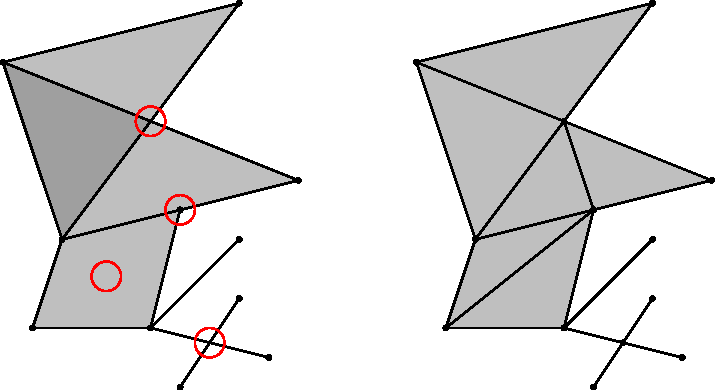
\includegraphics{chapters/95-homologie/images/polyeder.pdf}
\caption{Aufbau eines zweidimensionalen Polyeders aus
verschiedenen Simplizes.
Die Schnittmenge zweier Simplizes muss ein Untersimplex beider Simplizes
sein.
Die roten Kreise im linken Bild weisen auf verschiedene Situationen
hin, wo das diese Bedingung nicht erfüllt ist.
In rechten Bild sind zusätzliche Simlizes hinzugefügt worden, um
die Bedingungen eines Polyeders zu erfüllen.
\label{buch:homologie:figure:polyeder}}
\end{figure}
Aus einzelnen Simplizes können jetzt kompliziertere geometrische
Objekte gebaut werden.
Ein Graph ist ein Beispiel für ein geometrisches Objekt, welches
als Vereinigung von 1-Simplizes entsteht.
Die Vereinigung ist aber nicht beliebig, vielmehr ist die Schnittmenge
zweier beliebiger 1-Simplizes immer entweder leer, eine Menge 
mit nur einem Vertex oder ein ganzes 1-Simplex.

Dies reicht aber nicht, wie Abbildung~\ref{buch:homologie:polyeder}
zeigt.
In einem Graphen dürfen sich Kanten nicht in einem inneren Punkt treffen,
sondern nur in Endpunkten.
Verallgemeinert auf höherdimensionale Simplizes kann man dies als die
Bedingung formulieren, dass die Schnittmenge zweier beliebiger
Simplizes immer Untersimplizes beider Simplizes sein müssen.
Wir fassen dies zusammen in der folgenden Definition.

\begin{definition}
\index{Polyeder}%
\index{Dimension eines Polyeders}%
\index{Polyeder, Dimension eines}%
Ein {\em Polyeder} ist eine Vereingung von endlich vielen Simplizes derart,
dass die Schnittmenge zweier beliebiger Simplizes immer ein Untersimplex
beider Simplizes ist.
Die {\em Dimension} des Polyeders ist die grösste Dimension der darin
enthaltenen Simplizes.
\end{definition}

Ein Graph ist nach dieser Definition ein eindimensionales Polyeder.
Die Mengen in der Abbildung~\ref{buch:homologie:figure:polyeder}
ist kein Polyeder, kann aber leicht zu einem Polyeder gemacht werden,
indem man einzelne Kanten mit zusätzlichen Punkten unterteilt.
Auch müssen die zweidimensionalen Simplizes aufgeteilt werden.

Die Abbildung~\ref{buch:homologie:figure:polyeder} zeigt auch, dass
die Darstellung einer Punktmenge als Polyeder nicht eindeutig ist.
Man kann die Kanten und Flächen jederzeit weiter unterteilen, ohne
dass sich die Gestalt der gesamten Menge dadurch ändert.

\subsection{Triangulation
\label{buch:subsection:triangulation}}
Unser Ziel ist, geometrische Objekte besser verstehen zu können.
Dabei sind uns Deformationen ja sogar Knicke egal, es interessiert uns
nur die ``Gestalt'' des Objekts.
Entfernungen zwischen Punkten sind ebenfalls von untergeordneter 
Bedeutung, da sie bei Deformation nicht erhalten bleiben.
Der Begriff des ``topologischen Raumes'' fasst diese Ideen mathematisch
präzise ein, eine genaue Definition würde aber an dieser Stelle zu weit
führen.
Stattdessen beschränken wir uns auf eine Klasse von Punktmengen, die man
mit Simplizes beschreiben kann.

Ein topologischer Raum zeichnet sich durch einen Nachbarschaftsbegriff
von Punkte aus, der erlaubt zu definieren, was eine stetige Abbildung ist.
Ein stetige Abbildungen bildet nahe beeinander liegende Punkte wieder
auf nahe beeinander liegende Punkte ab.
Dass nahe liegende Punkte nicht plötzlich auf weit auseinander liegende
Punkte abgebildet werden gibt die Intuition wieder, dass Deformationen
möglich sein sollen, dass der Raum dabei aber nicht ``reissen'' darf.
Zwei topologische Räume $X$ und $Y$ können daher als ``gleichgestaltig''
betrachtet werden, wenn es zwei stetige Abbildungen $f\colon X\to Y$
und $g\colon Y\to X$ gibt, die zu einander invers sein.
Oder wenn sich $X$ stetig auf $Y$ abbilden lässt, so dass auch die
Umkehrabbildung stetig ist.
Eine solche Abbildung heisst ein {\em Homöomorphismus}, die beiden Räume
$X$ und $Y$ heissen {\em homomorph}.

Eine Kugel ist natürlich kein Polyeder, aber sie kann leicht homöomorph
auf ein dreidimensionales Simplex abgebildet werden.

\begin{beispiel}
Sei $T$ ein reguläres Tetraeder mit den Ecken auf der dreidimensionalen
Einheitskugel $B^3$.
Für jeden Richtungsvektor $x\ne 0$ sei $l(x)$ Entfernung vom Mittelpunkt des
Tetraeders bis zum Durchstosspunkt einer Geraden durch den Mittelpunkt
mit Richtungsvektor $x$ durch die Oberfläche des Tetraeders.
Dann sind die Abbildungen
\[
f\colon
T\to B^3
:
x \mapsto\begin{cases}
\displaystyle
\frac{x}{l(x)}&\quad\text{für $x\ne 0$}\\
0&\quad\text{für $x=0$}
\end{cases}
\qquad\text{und}\qquad
g\colon
B^3\to T
:
x \mapsto\begin{cases}
l(x) x&\quad\text{für $x\ne 0$}\\
0&\quad\text{für $x=0$}
\end{cases}
\]
zueinander inverse stetige Abbildungen oder Homöomorphismen.
\end{beispiel}

Im Folgenden sollen daher nur solche topologischen Räume untersucht werden,
die homöomorph sind zu einem Polyeder.
Man nennt die homöomorphe Abbildung eines Polyeders auf so einen Raum
auch eine Triangulation.
Durch Unterteilung der Simplizes in kleiner Simplizes kann eine solche
Triangulation beliebig verfeinert werden.






